In this paper, we conduct experiments on three widely used 
KGQA datasets, and we also construct our own GraphWalkerBench to further study the agent's capability to generalize to unseen structures: 

\textbf{WebQSP.} WebQSP is a foundational KGQA benchmark designed to evaluate a model’s ability to answer simple, fact-based questions that typically require retrieving a single fact from the knowledge graph. The dataset provides full SPARQL queries for its questions, which are executed against Freebase.

\textbf{CWQ.} CWQ extends the complexity beyond WebQSP by introducing questions that require compositional reasoning. These questions often involve multiple constraints, conjunctions, and superlatives, necessitating multi-hop or multi-relation inference paths on the Freebase knowledge graph.
The dataset is annotated with complex SPARQL queries that reflect these reasoning structures.

\textbf{GrailQA.} GrailQA is a large-scale dataset built on Freebase that is designed to evaluate the generalization capabilities of KGQA models across three distinct levels: i.i.d., compositional, and zero-shot. This structure allows for a fine-grained analysis of a model’s ability to handle previously seen patterns (i.i.d.), new combinations of seen patterns (compositional), and entirely new domains and relations (zero-shot).
Significantly, the zero-shot split in GrailQA evaluates the model’s ability to generalize to unseen query compositions. 




\textbf{GraphWalkerBench.}
GraphWalkerBench consists of 1766 queries covering a diverse set of reasoning 
structures, including 736 multi-hop compositions and 1030 conjunction patterns. 
As detailed in Table~\ref{tab:graphwalkerbench}, it specifically includes 
single-path composition queries (3-hop, 4-hop, and 5-hop) and multi-path 
conjunction queries (2I, IP, and PI), providing a balanced testbed for 
evaluating both depth and compositional complexity.

\begin{table}[htbp]
  \centering
  \small
  \setlength{\tabcolsep}{8pt}
  \caption{Structure distribution of GraphWalkerBench.}
  \label{tab:graphwalkerbench}
  \begin{tabular}{l ccc ccc c}
    \toprule
    \multirow{2}{*}{\textbf{Structure Type}} & \multicolumn{3}{c}{\textbf{Composition}} & \multicolumn{3}{c}{\textbf{Conjunction}} & \multirow{2}{*}{\textbf{Total}} \\
    \cmidrule(lr){2-4} \cmidrule(lr){5-7}
    & \textbf{3-hop} & \textbf{4-hop} & \textbf{5-hop} & \textbf{2I} & \textbf{IP} & \textbf{PI} & \\
    \midrule
    \textbf{Count} & 347 & 209 & 180 & 344 & 337 & 349 & 1766 \\
    \bottomrule
  \end{tabular}
\end{table}


\begin{figure}[htbp]
    \centering
    \begin{minipage}[t]{0.48\linewidth}
        \centering
        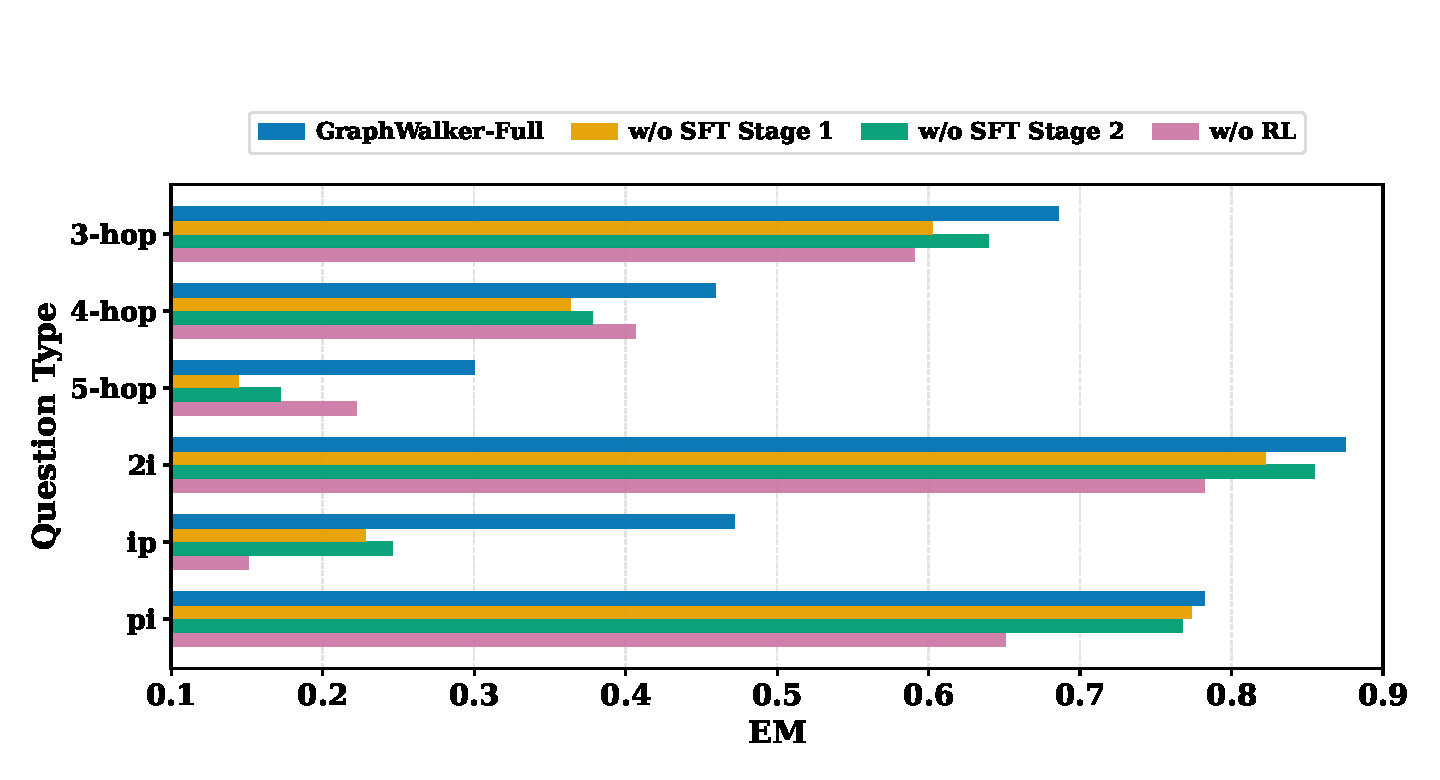
\includegraphics[width=\linewidth]{figures/gwbench_em_grouped_barh.pdf}
    \end{minipage}
    \hfill
    \begin{minipage}[t]{0.48\linewidth}
        \centering
        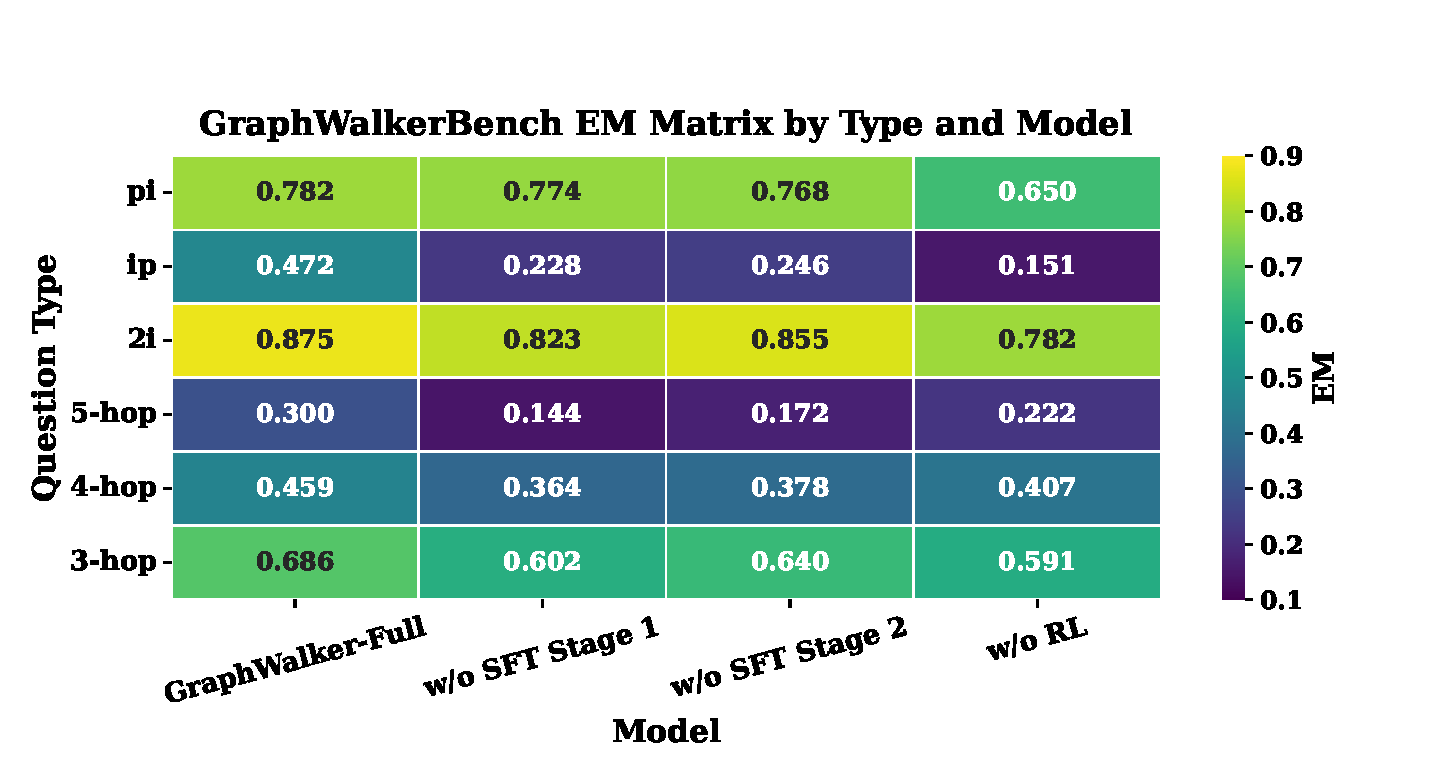
\includegraphics[width=\linewidth]{figures/gwbench_em_heatmap.pdf}
    \end{minipage}
    \caption{Fine-grained EM performance on GraphWalkerBench across question 
    types and ablation variants. \textbf{Left}: grouped bar chart. 
    \textbf{Right}: heatmap. IP and PI are unseen conjunction structures 
    not present in GraphSynth training data.}
    \label{fig:gwbench_analysis}
\end{figure}


In Figure~\ref{fig:gwbench_analysis}, we present a fine-grained breakdown of EM performance across question types on GraphWalkerBench. 
\textbf{GraphWalker-Full} achieves the highest EM across nearly all types, with particularly strong generalization to unseen conjunction structures (IP and PI), confirming that GraphSynth is the primary driver of structural 
generalization. Removing either SFT stage or RL consistently degrades performance, with severe drops observed on IP queries and deep multi-hop compositions, corroborating the findings in Table~\ref{tab:zeroshot}.